\begin{figure}[htbp]
\centering
\begin{tikzpicture}[schema base]
\node[schema titolo] at (0,0.3) {Stessa immagine, due associazioni documentali diverse};
\path[schema pannello] (0,-0.2) rectangle (5,-6.65);
\node[schema etichetta,text width=4.6cm] at (2.5,-0.7) {\textbf{WM250, pagina 10}\newline Figura 11 del manuale};
\node[inner sep=0] at (2.5,-3.4)
  {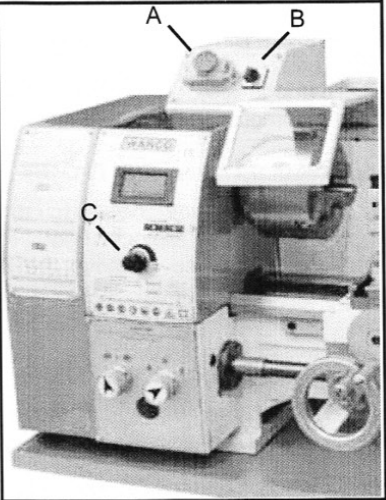
\includegraphics[width=3.1cm]{figure/asset/v4/paddle-image-0010-0001.png}};
\node[schema nota,text width=4.4cm] at (2.5,-6)
  {Asset originale};
\node[schema esterno,text width=7.7cm,minimum height=1.8cm] (padre) at (10.6,-1.45)
  {\textbf{Padre salvato in manual.json}\\\enquote{8. Cross Slide Lock}\\Associazione canonica non aggiornata};
\node[schema blocco,text width=7.7cm,minimum height=2.9cm] (contesto) at (10.6,-5)
  {\textbf{Contesto nella richiesta 0004}\\[4pt]
  A -- Emergency Button ON/OFF Switch\\
  B -- Change-over Switch\\
  C -- Variable Speed Control Switch\\[4pt]
  Sezioni che richiamano la Figura 11};
\draw[schema freccia,draw=schemaOcra] (5,-1.45) -- (padre.west);
\draw[schema freccia,draw=schemaBlu] (5,-5) -- (contesto.west);
\node[schema nota,text width=14.3cm] at (7.5,-7.45)
  {Il contesto della richiesta è più pertinente, ma il capitolo padre non viene corretto.};
\end{tikzpicture}
\caption{Due associazioni per \texttt{paddle-image-0010-0001}, da \texttt{manual.json} e dalla richiesta OCR \texttt{0004}. I richiami contestuali non sono nuovi capitoli. La discrepanza è ispezionabile anche se la caption viene esclusa per lunghezza.}
\label{fig:gerarchia-contesto-wm250}
\end{figure}